%\chapter*{Introduction}
\chapter{Introduction}
%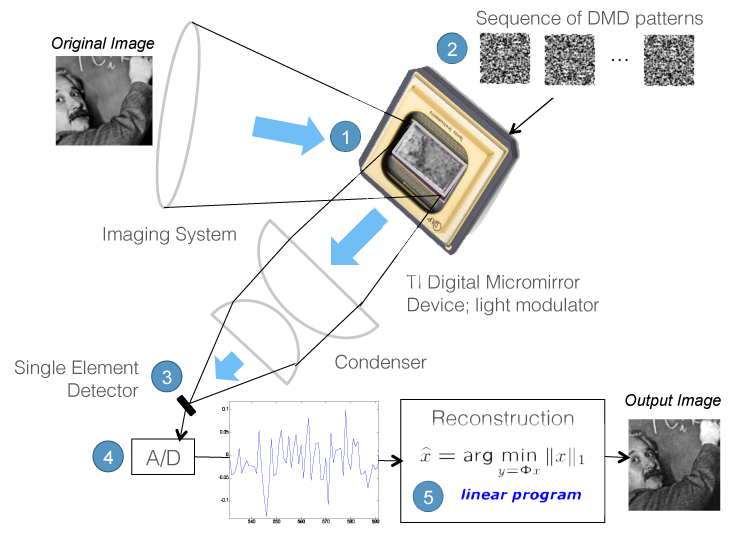
\includegraphics{Img1.png}
%\addcontentsline{toc}{chapter}{Introduction}
\section{Motivation}
Compressed sensing (CS) is a novel technique based on the discoveries done by Candes \textit{et al}. \cite{CandesR07} and Donoho \cite{Donoho01}. They showed that as long as certain conditions are met, a signal can be fully recoverd from a small number of measurements. Due to this fact, CS is suitable for many Signal Processing (SP) applications and specifically image processing. An example of this are the publications made by Duearte \textit{et al}. and Wakin \textit{et al}. \cite{duarte2008single,wakin2006architecture}. In their work they explained their ideas for architecting an imaging sensor capable of sampling and compressing the signal at the same time. Such a sensor offers the advantage of taking less samples than those needed by conventional sensors and there is no extra compression phase after the measurements are taken, thereby saving computation workload. As a result, the industry and the research community have been interested and actively worked during the last years in order to design sensors capable of giving both better energy efficiency as well as good algorithms capable of yielding high quality for the recovered images. Unfortunately, everything comes with a cost and recovering the original image from such compressed measurements is a problem that has high complexity and computationally expensive to solve. These problems are commonly referred to as inverse problems, since one tries to recover a signal from under-sampled measurements, which translates into trying to find a solution to an under-determined system. \

Many algorithms have been proposed for image reconstruction, among the most widely known and recognized one can find \cite{metzler2014denoising,dong2014compressive, li2013efficient,mun2009block,chen2011compressed,fowler2011multiscale}. Nevertheless, most of them suffer from the same disadvantages because they follow the most general approach for the reconstruction process. First, they solve an optimization problem, which implies the use of iterations until a possible solution is obtained. Because of that, those algorithms are called iterative. Furthermore, they may need up to 10 minutes to reconstruct only one image. Second, they only focus on obtaining raw pixel values that, hopefully, will correspond to the original image. That makes such algorithms not useful for other common tasks like object detection and segmentation. Although those algorithms are not fast and therefore not suitable for real-time applications, they render reconstructed images with high quality and good visual impact. Designing algorithms that can reconstruct images from compressed measurements in a simpler faster way while keeping or increasing the final quality of the image is still an active topic for research and one of the major motivations for this thesis. \

Another justification for this thesis is the state-of-the-art results that Deep Neural Networks (DNNs) \cite{lecun2015deep} have proved for several image processing tasks like classification \cite{krizhevsky2012imagenet}, image denoising \cite{burger2012image} and superresolution \cite{dong2014learning}. Based on the promising performance of those examples, applying DNNs for reconstructing images from compressed measurements seems to be another application that should be investigated. Namely, we focus on the use of Convolutional Neural Networks (CNNs) for the afore mentioned task and because of its nature the reconstruction process may take less time and the quality as well as the visual impact of the images could also be preserved or even increased.  

In this thesis a different method for image reconstruction that does not follow the conventional approach is proposed, that is we do not try to find a solution for an optimization problem. As a result, this is a non-iterative solution for recovering images from compressed measurements. In order to reconstruct the image we exploit the proven capacity of CNNs for image processing tasks. Several network architectures are evaluated and compared with iterative methods in terms of time and final quality of the reconstructed image.

\section{Outline}
The thesis follows this organization: \

{\bfseries Chapter 2 - Theoretical foundations}  introduces the important background in compressed sensing, deep learning and CNNs. It also presents the common problems that are faced when trying to recover images from compressed measurements using traditional algorithms. \\
{\bfseries Chapter 3 - Implementation methodology} gives an overview of the datasets and tools that are used in order to build and implement the neural network. It also explains the data preparation and post processing that yields the final outcome. We also describe the CNN's we have devised in order to recover images from compressed measurements. \\
{\bfseries Chapter 4 - Evaluation} shows the reconstruted images using our CNN and explains the training procedure. We also make a comparison between state-of-the-art iterative algorithms for the recovery process against the proposed method using CNNs. The evaluation is made in terms of the speed and quality. It also explains the differences between several network architectures.  \\
{\bfseries Chapter 5 - Conclusion} states the lessons learned throughout the development of the thesis as well as the future work that could lead to better results and extend its application. \\
